Al fine di valutare la reattivit\`{a} del sensore coppia-forza, \`{e} stato condotto un esperimento per esaminare la capacit\`{a} del 
sensore di rilevare rapidamente una variazione istantanea della forza. 
Tale variazione improvvisa \`{e} stata simulata 
tagliando un filo che sosteneva un oggetto appeso al sensore. La misurazione rilevata a seguito del taglio  
deve mostrare una variazione \textbf{proporzionale al peso dell'oggetto}.
In questo esperimento, \`{e} stato attaccato al sensore un filo con appeso un oggetto di 0.155 Kg. 
Il braccio \`{e} stato posizionato in modo tale che la forza peso gravasse solo su un asse del sensore alla volta, cosicch\`{e} 
il valore rilevato dopo il taglio fosse compatibile con il peso dell'oggetto precedentemente attaccato. 
In Figura \ref{fig:setup_z}, viene mostrato il setup per l'esperimento lungo l'asse z. 
\begin{figure}[H]
    \centering
    \begin{subfigure}[b]{0.4\textwidth}
        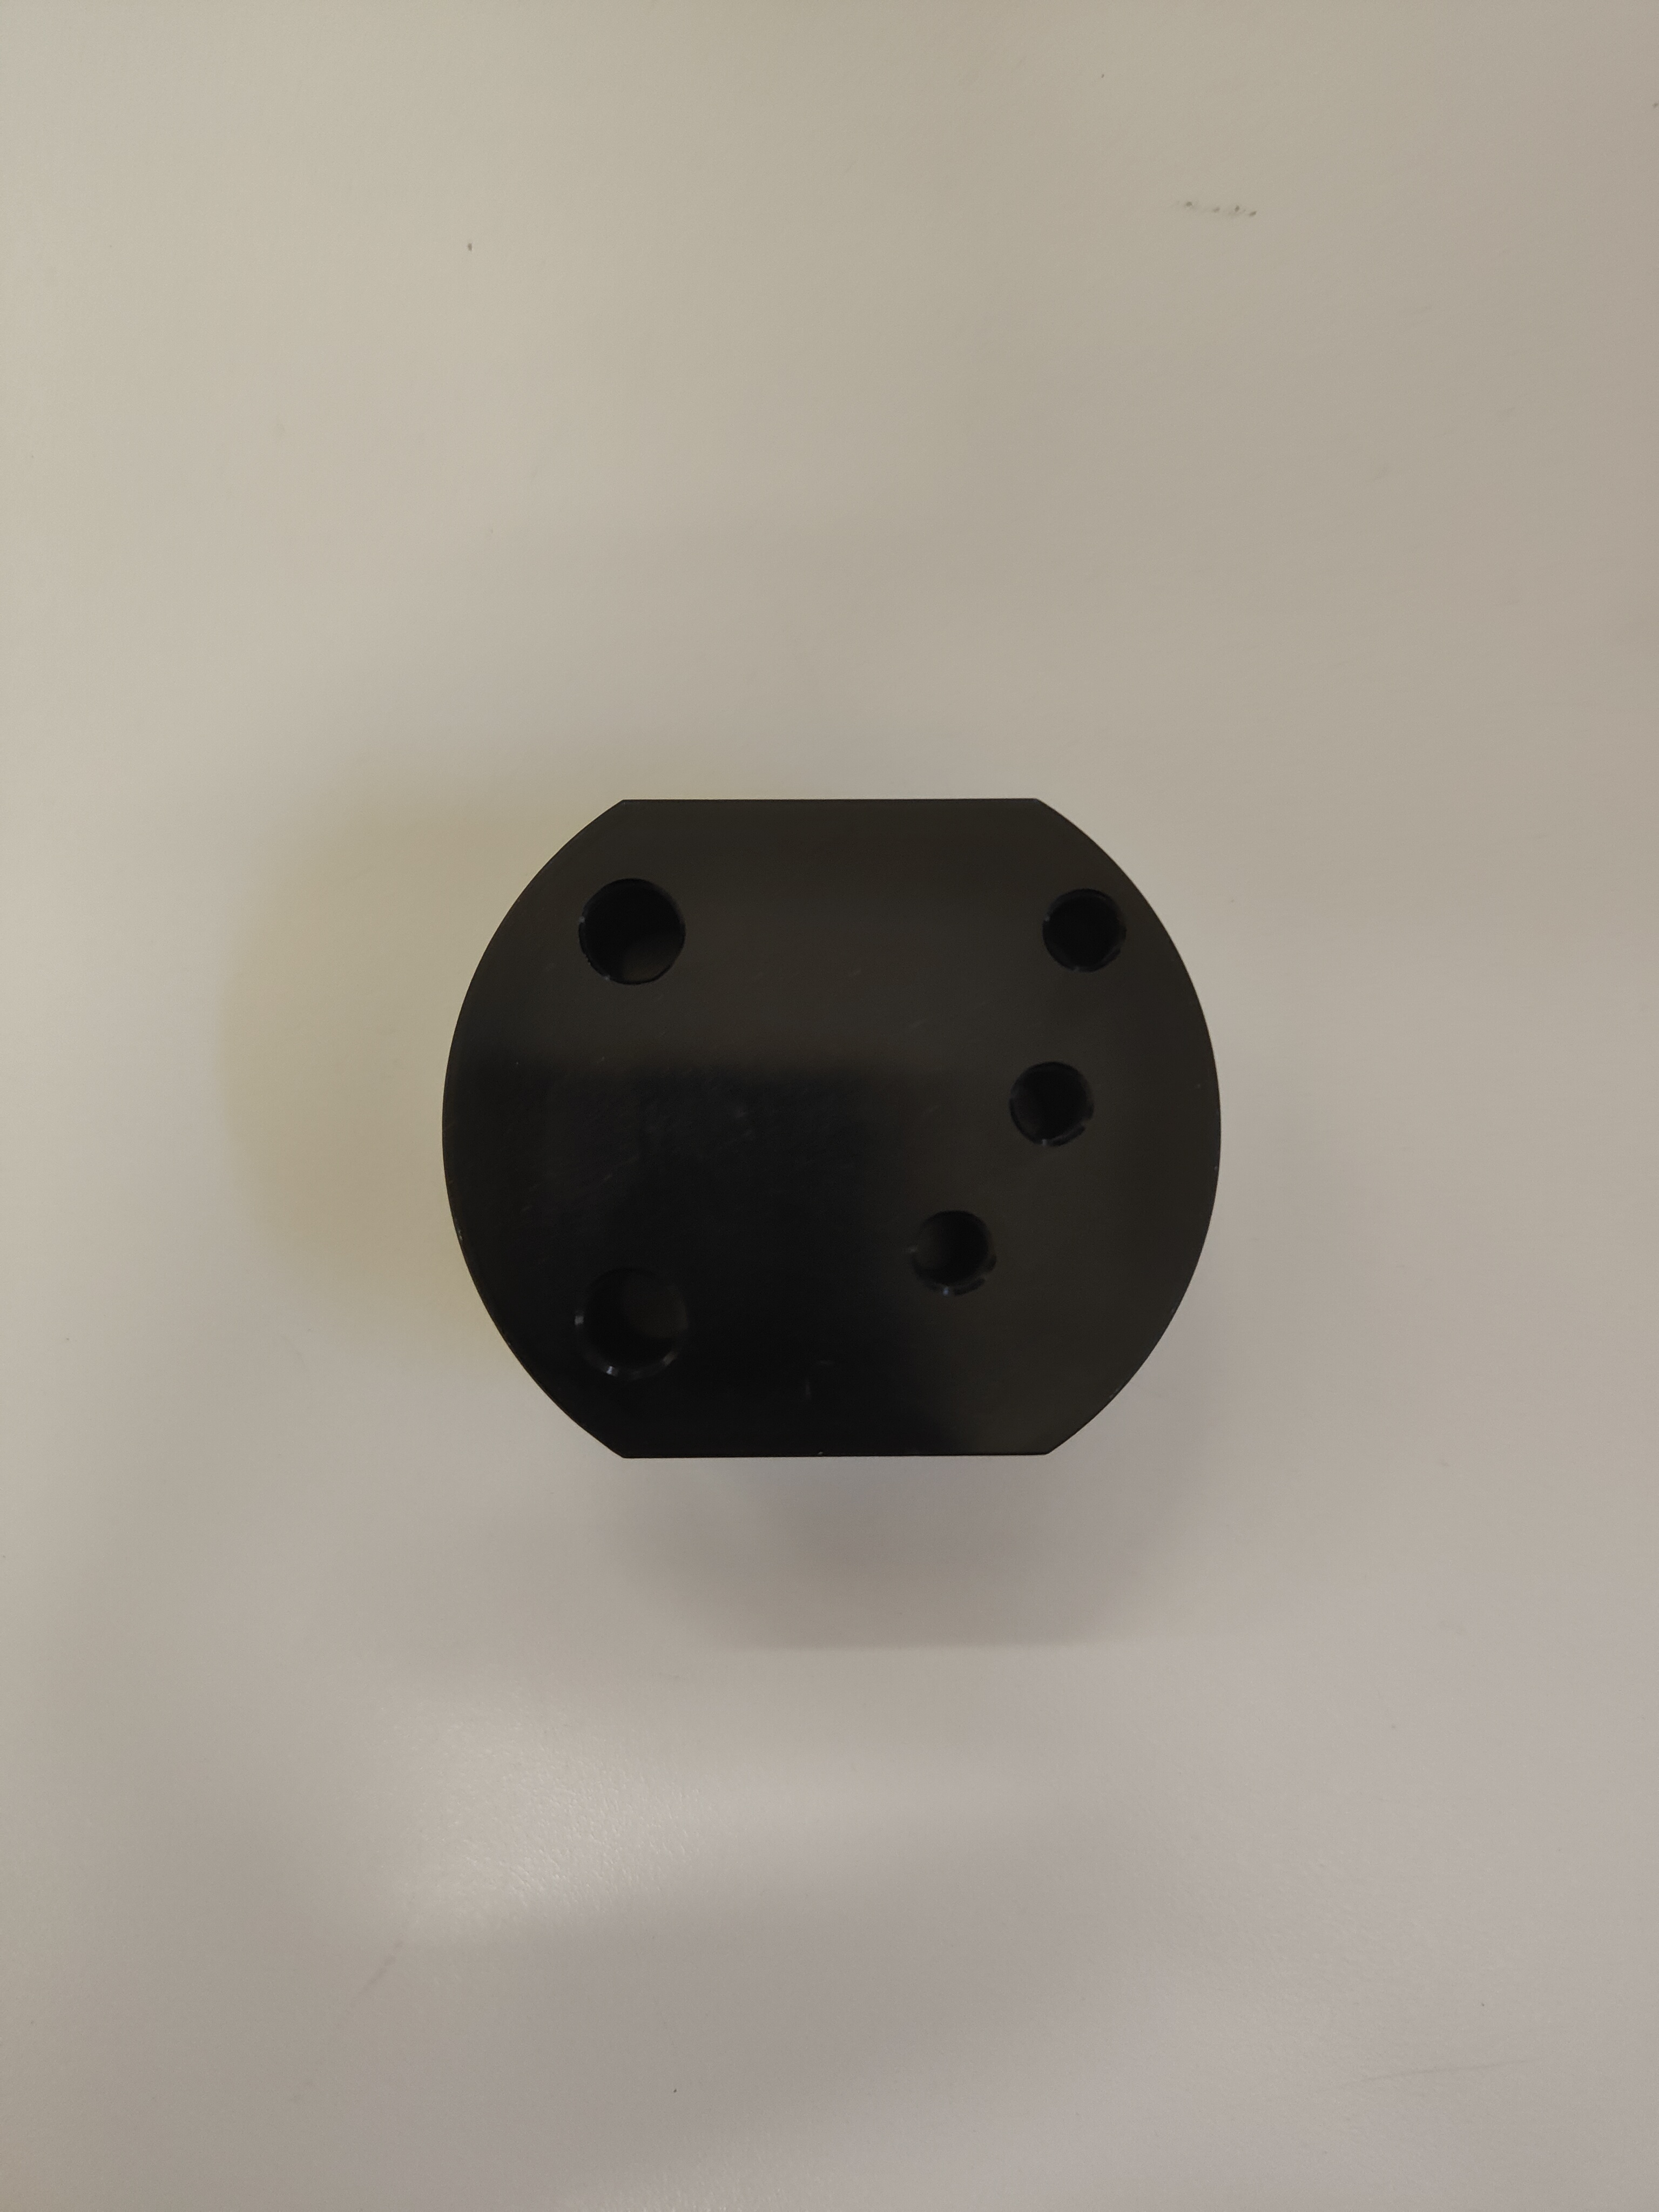
\includegraphics[width=\textwidth]{images/object.jpg}
        \label{fig:object}
    \end{subfigure}
    \qquad
    \begin{subfigure}[b]{0.4\textwidth}
        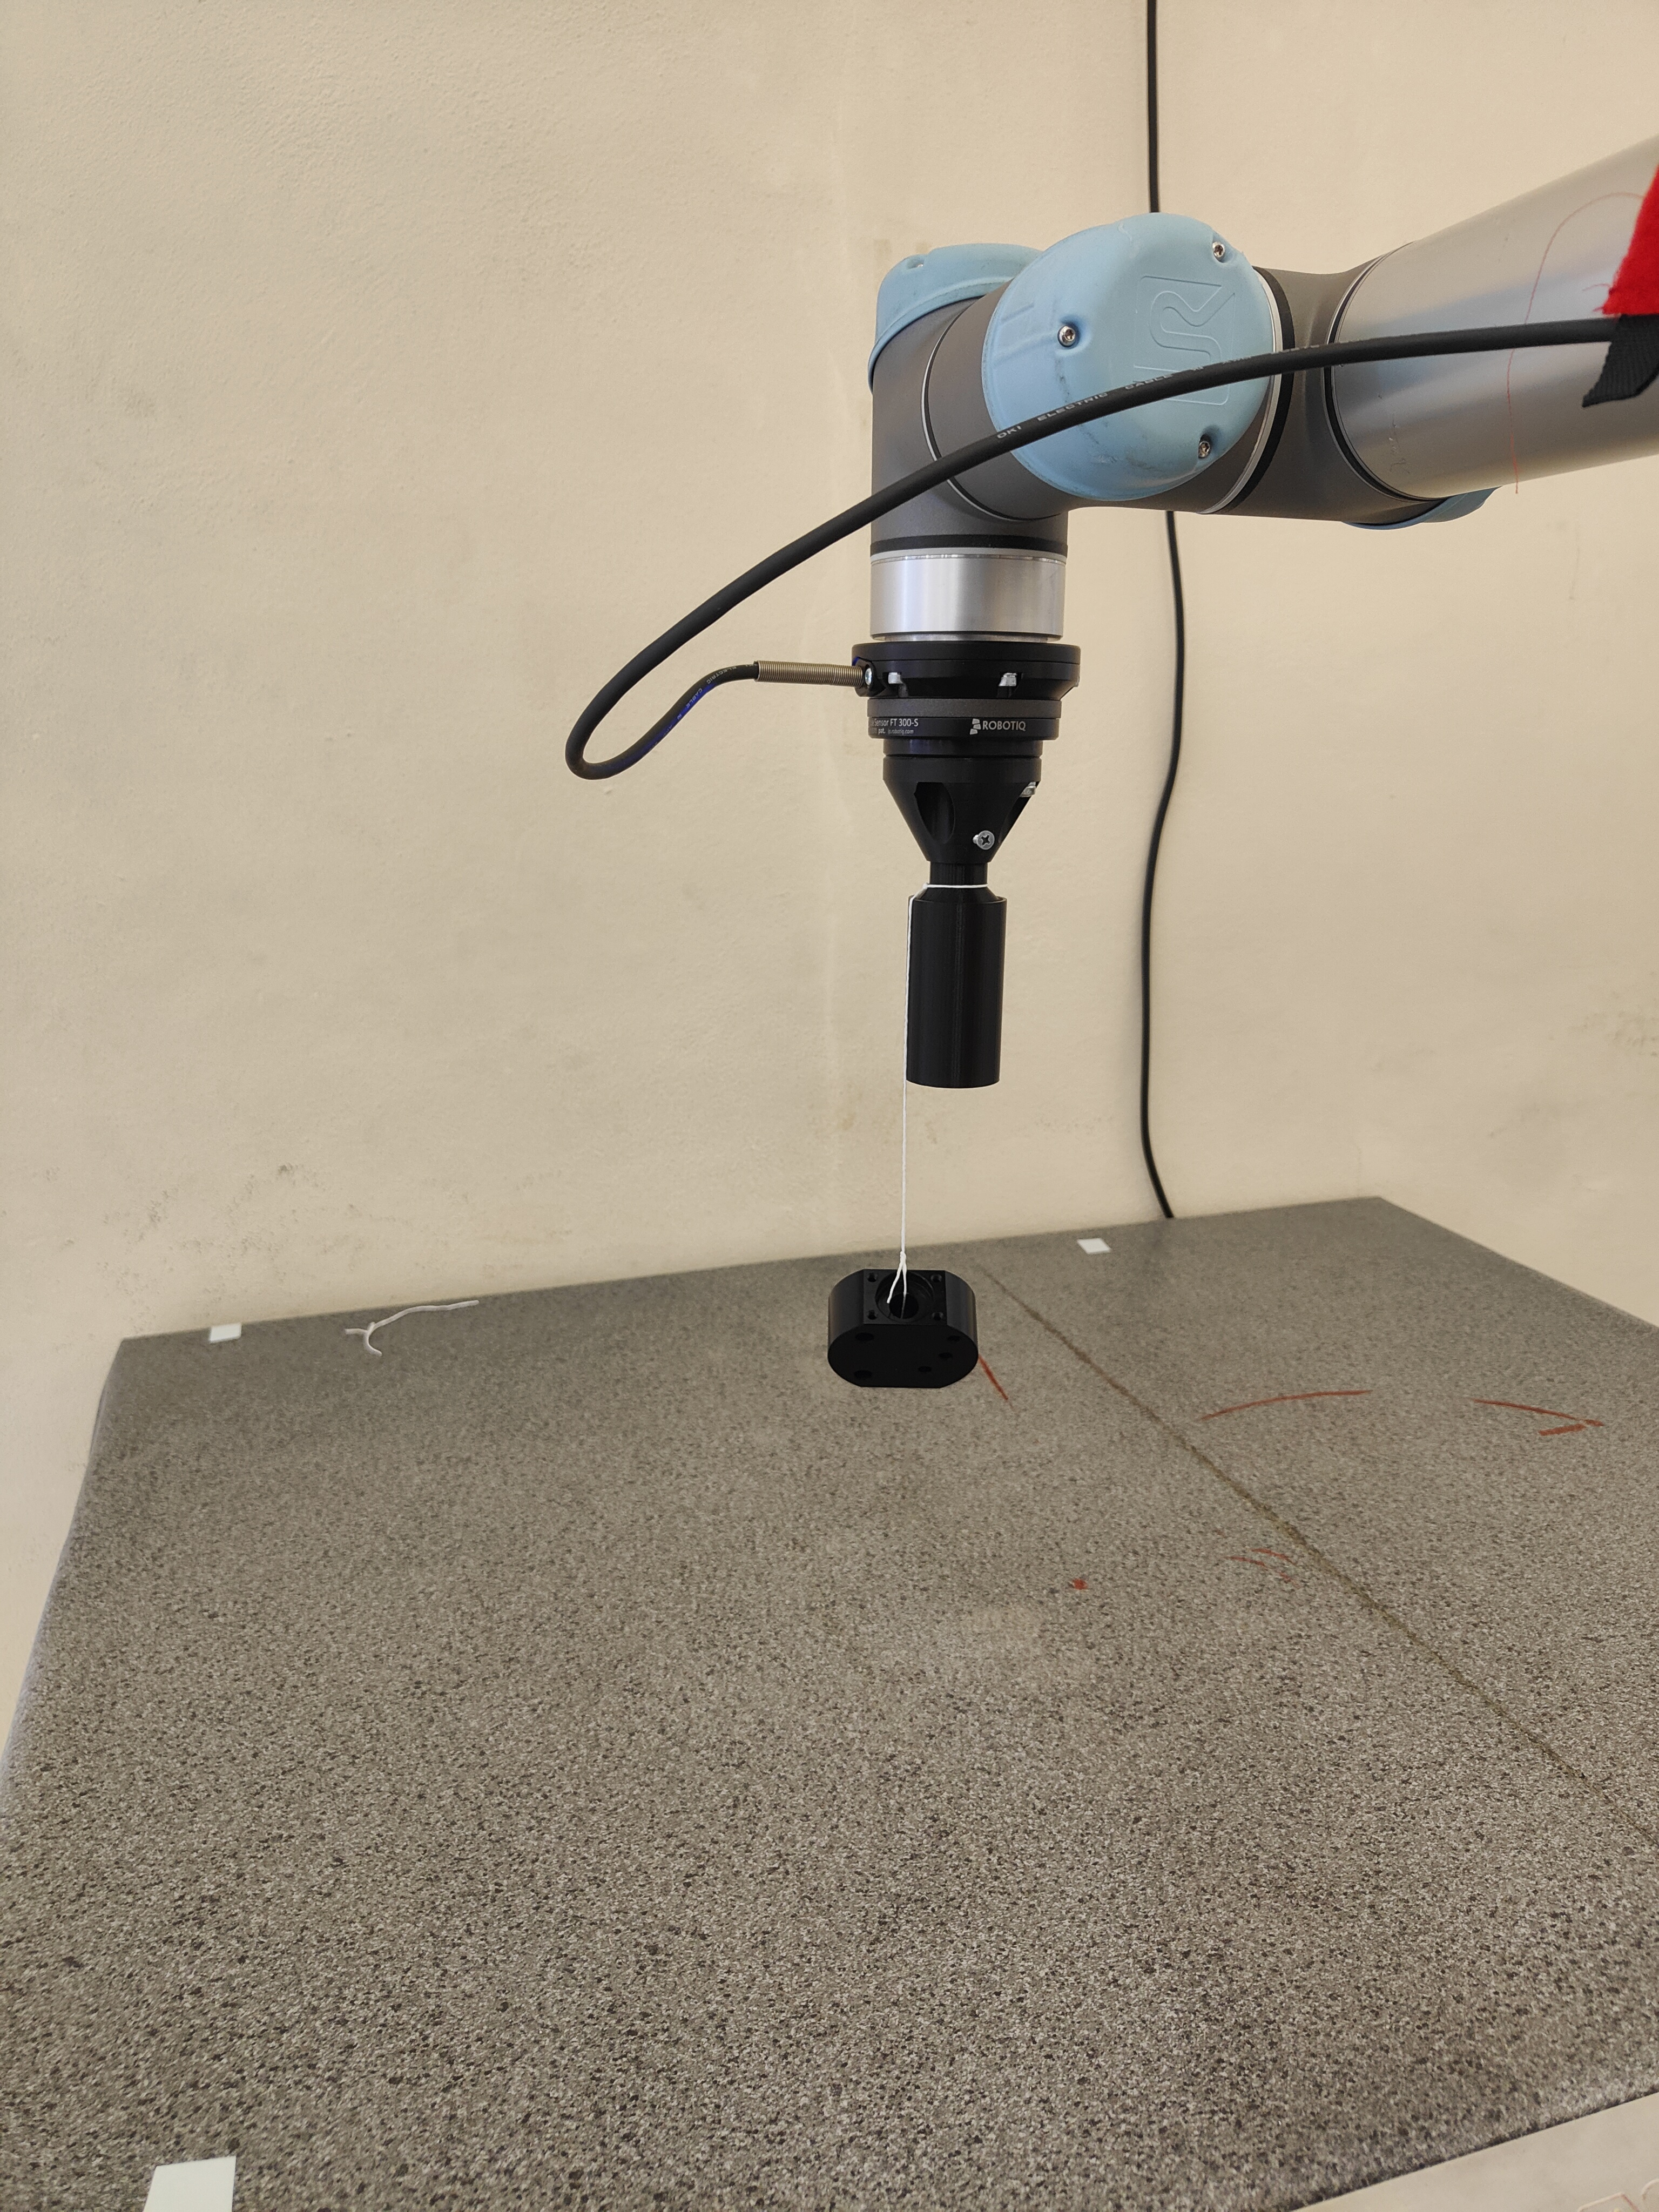
\includegraphics[width=\textwidth]{images/setup_z.jpg}
        \label{fig:setup}
    \end{subfigure}
    \caption{Setup sperimentale per l'analisi della reattivit\`{a}. A sinistra, l'oggetto di metallo utilizzato, 
    a destra l'oggetto collegato con un filo al robot (forza peso che grava sull'asse z del sensore)}\label{fig:setup_z}
\end{figure}
Dopo aver azzerato il sensore, per verificarne la reattivit\`{a}, il filo \`{e} stato tagliato di netto. 
Il taglio del filo \`{e} un ottimo modo per `simulare' un cambiamento di forza istantaneo.
\begin{figure}[H]
    \centering
    \includegraphics*[width=0.85\textwidth]{images/z_cut.png}
    \caption{Andamento taglio del filo misurato lungo l'asse z del sensore coppia-forza}
    \label{fig:z_cut}
\end{figure}
In Figura \ref{fig:z_cut} viene mostrato l'andamento della forza rilevata dal sensore lungo l'asse z. 
Si pu\`{o} notare che, fino a quando il filo \`{e} attaccato al sensore, la forza rilevata \`{e} circa zero. 
Questo perch\'{e} il sensore \`{e} stato azzerato quando l'oggetto era gi\`{a} stato appeso al sensore. 
Nel momento in cui avviene il taglio, il grafico si allinea istantaneamente al peso reale dell'oggetto, 
ossia circa 1.5 N (il valore previsto dovrebbe essere $0.155 \text{ Kg} \cdot 9.81 \frac{\text{N}}{\text{Kg}} = 1.52055 \text{ N}$).
Tale esperimento \`{e} stato ripetuto anche per gli altri due assi, confermando lo stesso valore indicativo di -1.5 N.
\begin{figure}[H]
    \centering
    \includegraphics*[width=0.45\textwidth]{images/setup_x.jpg}
    \caption{Setup sperimentale per l'analisi della reattivit\`{a} lungo l'asse x del sensore coppia-forza}
    \label{fig:setup_x}
\end{figure}
Muovendo il robot nella configurazione mostrata in Figura \ref{fig:setup_x}, la forza peso dell'oggetto grava univocamente sull'asse x 
del sensore. 
Ruotando l'end effector di 90° si ottiene il setup equivalente per l'asse y.
I risultati vengono mostrati in Figura \ref{fig:x_cut} e \ref{fig:y_cut}.
\newpage 
\begin{figure}[H]
    \centering
    \includegraphics*[width=0.85\textwidth]{images/x_cut.png}
    \caption{Andamento taglio del filo misurato lungo l'asse x del sensore coppia-forza}
    \label{fig:x_cut}
\end{figure}
\begin{figure}[H]
    \centering
    \includegraphics*[width=0.85\textwidth]{images/y_cut.png}
    \caption{Andamento taglio del filo misurato lungo l'asse y del sensore coppia-forza}
    \label{fig:y_cut}
\end{figure}
A differenza di quanto riportato nei primi due grafici, l'andamento della forza rilevata lungo l'asse y, presenta un picco 
anomalo dovuto al taglio non sufficientemente netto del filo.
